% Use nolinenumbering to suppress line numbers in this draft
\documentclass[nolinenumbering]{thesisdesign}

% Packages not already loaded by thesisdesign.cls
\usepackage[utf8]{inputenc}
\usepackage{enumitem}
\usepackage{array}
\usepackage{multirow}
% natbib for \citep / \citet author-year citations
\usepackage{natbib}

% ── Author / title metadata (thesisdesign.cls commands) ──────────
\thesistitle{Bridging the Stability-Plasticity Dilemma in Anti-UAV Systems:\\
Incremental Adaptation from Standard RGB to Tiny Thermal Infrared Targets}
\thesissubtitle{Chapter: Methodology and Experimental Setup}
\thesisdate{\today}
\authorname{Giang Nguyen}
\authoremail{kdgiang.nguyen02@gmail.com}
\authorid{Student ID: XXXXXXXX}
\uvasupervisorname{[Supervisor Name]}
\uvasupervisoraffiliation{University of Amsterdam}
\uvasupervisoremail{supervisor@uva.nl}
% ─────────────────────────────────────────────────────────────────

\begin{document}
\maketitle

% ─────────────────────────────────────────────────────────────────
\section{Research Design}
\label{sec:research_design}
% ─────────────────────────────────────────────────────────────────

This thesis follows a sequential empirical evaluation design. The core claim is that scale-distribution shift induces greater catastrophic forgetting in the penultimate feature space of a neural detector than a cross-modality shift does, given a fixed memory budget. To test this, the system is trained through a two-task curriculum: Task T1 adapts a source-domain RGB detector to a thermal infrared (TIR) target domain, and Task T2 subsequently shifts that TIR-adapted detector to extreme tiny-scale TIR targets. The degree of forgetting on T1 is measured after T2 training. This structure mirrors the sequential protocol used in continual learning benchmarks such as Split-CIFAR \citep{rebuffi2017icarl}, but applied to a real-world anti-UAV detection setting with authentic distribution shifts rather than artificially partitioned class sets.

The design differs from most prior work in two respects. First, existing UDA studies for drone detection---such as the Foggy Drone Teacher \citep{zheng_foggy_2025} and TTSDA-YOLO \citep{zhang_ttsda-yolo_2025}---treat domain adaptation as a static, one-off transfer and do not measure what is destroyed in the source domain when the model is subsequently fine-tuned. Second, existing anti-UAV benchmarks such as Anti-UAV410 \citep{bohuang_410} and CST Anti-UAV \citep{xie2025cstantiuavthermalinfrared} are evaluated in isolation. This thesis is the first to chain them into a shared model's training history and measure the resulting stability-plasticity trade-off quantitatively.


% ─────────────────────────────────────────────────────────────────
\section{Methodology}
\label{sec:methodology}
% ─────────────────────────────────────────────────────────────────

The proposed system is composed of three interdependent modules. Module~1 performs unsupervised domain adaptation from RGB to TIR using a Teacher-Student framework. Module~2 applies continual learning with a rehearsal buffer to preserve T1 knowledge during T2 fine-tuning, using a novel Scale-Stratified Herding strategy. Module~3 fuses spatial appearance and temporal motion signals at inference time, gated by an evidential uncertainty head that suppresses the appearance branch during thermal crossover. Each module is described below in terms of what it does, how it does it in this specific context, and why it was chosen over plausible alternatives.


% ─────────────────────────────────────────────────────────────────
\subsection{Module 1: Teacher-Student Unsupervised Domain Adaptation}
\label{sec:uda}
% ─────────────────────────────────────────────────────────────────

The T1 shift---from RGB to thermal infrared---is addressed without target-domain annotations. The Anti-UAV-RGBT dataset \citep{jiang_anti-uav_2023} provides temporally paired RGB and IR video streams of the same scene, recorded simultaneously. This pairing is the key enabling condition. A teacher model is first trained on the labelled RGB stream to convergence, where ground-truth bounding boxes are available. The teacher's weights are then frozen. A student model, which will operate on the IR stream at deployment, is initialized from the same weights and then fine-tuned on the unlabelled IR stream, supervised only by the teacher's predictions. The consistency loss penalizes divergence between teacher and student detections on the same spatial region as seen through different sensors. Because both streams observe the same drone at the same moment, the teacher's predictions serve as a reliable soft label signal without any IR annotation effort.

This approach is chosen over adversarial domain alignment methods such as DANN because adversarial training introduces a gradient reversal layer that can be unstable when the domain gap is large---which it is here, given that IR and RGB have fundamentally different noise statistics and contrast mechanisms. Teacher-Student consistency training, by contrast, is a unidirectional and stable objective. \citet{zheng_foggy_2025} demonstrated precisely this advantage for drone detection under foggy degradation, and \citet{luangluewut_investigating_2025} confirmed that the consistency framework is computationally lightweight enough for CPU-based edge deployment. The paired-stream structure of Anti-UAV-RGBT makes the teacher signal unusually reliable compared to typical UDA scenarios, where source and target are collected independently.


% ─────────────────────────────────────────────────────────────────
\subsection{Module 2: Continual Learning with Scale-Stratified Herding}
\label{sec:cl}
% ─────────────────────────────────────────────────────────────────

After T1 training converges, the model is fine-tuned on the CST Anti-UAV dataset \citep{xie2025cstantiuavthermalinfrared}, which contains targets that are predominantly sub-10 pixels in diameter. Without memory protection, this fine-tuning causes catastrophic forgetting: the feature extractor specializes for tiny targets and loses the geometric invariants needed to detect standard-scale drones, exactly the stability-plasticity dilemma described by \citet{deng_unlocking_2025}.

The protection mechanism is a penultimate-feature rehearsal buffer, following the memory constraint established by \citet{chaudhry2019tiny}: the buffer is limited to a total capacity equivalent to 10\% of the model's parameter count, expressed as a number of stored feature vectors. Sampling into the buffer uses the Herding strategy from iCaRL \citep{rebuffi2017icarl}, which selects samples whose penultimate-layer embeddings are closest to the mean embedding of their class, preserving the most representative geometric structure rather than storing random or peripheral examples.

The novel modification introduced in this thesis is Scale-Stratified Herding. Standard iCaRL herding treats all T1 samples uniformly, which in practice leads to a buffer dominated by large-target examples because they are the majority class in Anti-UAV410. When the T2 fine-tuning then shifts the model toward tiny targets, the buffer's large-target embeddings provide useful resistance---but offer no protection for the small or normal scale range, which can still drift. Scale-Stratified Herding partitions the buffer capacity proportionally across bounding box size categories (tiny, small, normal, large) using the COCO size boundaries (32, 96, and 192 pixels on the long side relative to a 640$\times$512 frame). Each stratum is herded independently, so the buffer's coverage of the embedding space reflects the scale distribution of T1 rather than the frequency distribution of the raw data. The hypothesis being tested is that this stratified geometry preservation will reduce the Forgetting Measure relative to a flat-herding baseline under the same memory budget.

This approach is justified by the theoretical analysis of \citet{deng_unlocking_2025}, who showed that rehearsal-based methods are provably effective when the replayed distribution matches the original task distribution in feature space. Stratifying by scale ensures precisely this: the replayed embeddings collectively span the full scale regime of T1 rather than over-representing one corner of it.


% ─────────────────────────────────────────────────────────────────
\subsection{Module 3: Bimodal Fusion with Evidential Gating}
\label{sec:fusion}
% ─────────────────────────────────────────────────────────────────

The backbone detector is YOLOMG \citep{guo_yolomg_2025}, a YOLOv5-based architecture extended with a second input channel: a pixel-level motion difference map (mask32) computed from consecutive frames. This dual-channel structure means the detector can draw on both spatial appearance information from the current IR frame and motion residual information from the temporal difference signal. At training time, these two signals are fused as concatenated channels in the early convolutional layers.

The motion difference maps require Global Motion Compensation (GMC) before they are useful. Camera ego-motion on an airborne platform induces apparent background motion that would otherwise overwhelm the small motion signature of a target drone. GMC is applied via the Enhanced Correlation Coefficient (ECC) algorithm \citep{evangelidis2008parametric}, which estimates a homography matrix aligning consecutive frames by maximizing the correlation coefficient between them. This frame-to-frame alignment removes the global background shift, leaving only the object-relative motion as the residual signal fed to the temporal branch. This is the same View-Centric GMC strategy employed by \citet{ji2026viewcentric} for multi-object tracking under extreme aerial ego-motion, adapted here to the single-object tiny-target setting.

The critical failure mode for purely appearance-based detection is thermal crossover: at certain ambient temperatures, the drone's radiometric signature matches the background, rendering the appearance branch uninformative or actively misleading. To handle this dynamically rather than with a static weight, the system adds an Evidential Head on top of the appearance branch output. Rather than producing a standard softmax probability, the evidential head treats the network's output as the parameters of a Dirichlet distribution over class probabilities \citep{sensoy2018evidential}. The vacuity---the total epistemic uncertainty, computed as the number of classes divided by the sum of the Dirichlet parameters---rises when the head has little evidence. High vacuity during thermal crossover is therefore a learnable, mathematically grounded signal that the appearance branch should be suppressed. The fusion gate down-weights the appearance branch proportionally to its vacuity and shifts reliance to the motion branch, which remains robust as long as the drone is moving relative to the camera.

This design choice is directly motivated by \citet{zhu_evidential_2023}, who demonstrated that explicit vacuity gating reduces identity switches (IDSW) during anti-UAV tracking by preventing the tracker from locking onto background noise during crossover events. The alternative---static or learned fixed-weight fusion---cannot adapt to crossover events at inference time without retraining. MC dropout or ensemble-based uncertainty is computationally too expensive for the real-time constraint of this application. The evidential formulation is a single forward pass and adds no inference latency beyond the head's own computation.


% ─────────────────────────────────────────────────────────────────
\section{Experimental Setup}
\label{sec:experimental_setup}
% ─────────────────────────────────────────────────────────────────


% ─────────────────────────────────────────────────────────────────
\subsection{Datasets}
\label{sec:datasets}
% ─────────────────────────────────────────────────────────────────

Four benchmark datasets are used, each assigned a specific role in the two-task curriculum. All four were audited empirically on the Snellius HPC cluster to verify sequence counts, frame totals, annotation formats, and bounding box size distributions before any training was conducted. The audit results are summarized in this section and visualized in Figures~\ref{fig:size_dist}, \ref{fig:visibility}, and \ref{fig:frame_counts}.

Anti-UAV-RGBT \citep{jiang_anti-uav_2023} is the T1 source domain. Each sequence contains two synchronized video streams---an infrared recording (\texttt{infrared.mp4}) and a visible RGB recording (\texttt{visible.mp4})---with per-frame bounding box annotations stored in \texttt{infrared.json}. The IR test split contains 85,374 frames with 98.6\% target visibility. The bounding box size distribution is dominated by large targets (68.4\%), with only 3.4\% of frames containing tiny or small targets (Figure~\ref{fig:size_dist}). This characterizes Anti-UAV-RGBT as a standard-scale IR detection corpus appropriate for establishing the T1 detection baseline before scale shift is introduced.

Anti-UAV410 \citep{bohuang_410} is the T1 target domain for UDA. It stores pre-extracted JPEG frames alongside per-sequence \texttt{IR\_label.json} annotation files. The dataset spans 438,397 frames across three splits: 213,995 training, 94,711 validation, and 129,691 test frames. The training split has 97.7\% target visibility and a scale distribution comparable to Anti-UAV-RGBT: 43.2\% large, 26.8\% normal, 27.5\% small, 2.5\% tiny. This confirms that T1 as a whole operates in a large-to-normal scale regime, which is the baseline the model must retain after T2 fine-tuning.

ARD100 provides ego-motion training data for the YOLOMG temporal branch. It contains 100 drone video sequences (65 training, 35 test) stored as MP4 files, with per-frame annotations in Pascal VOC XML format. The audit yielded 202,411 total annotated frames. Unlike the other three datasets, ARD100 is captured from a moving camera platform, giving it a scale distribution dominated by small targets (75.3\%) with significant ego-motion. ARD100 is used exclusively for generating the FD5 motion difference masks and is not part of the domain adaptation or continual learning curriculum.

CST Anti-UAV \citep{xie2025cstantiuavthermalinfrared} is the T2 target domain. It stores per-frame JPEG images with per-sequence annotations in \texttt{IR\_label.json} format. The full dataset spans 245,471 frames across three splits: 127,991 training, 45,305 validation, and 72,175 test frames. The scale distribution in the training split is strikingly different from T1: 73.6\% small, 20.5\% tiny, 5.9\% normal, and 0\% large. Additionally, 14.1\% of CST frames are annotated as occluded (thermal crossover conditions), compared to under 2.5\% in T1 datasets (Figure~\ref{fig:visibility}). This combination of extreme scale shift and elevated occlusion rates makes CST the primary stress-test for both the continual learning module and the evidential gating mechanism.

\begin{figure*}[t]
    \centering
    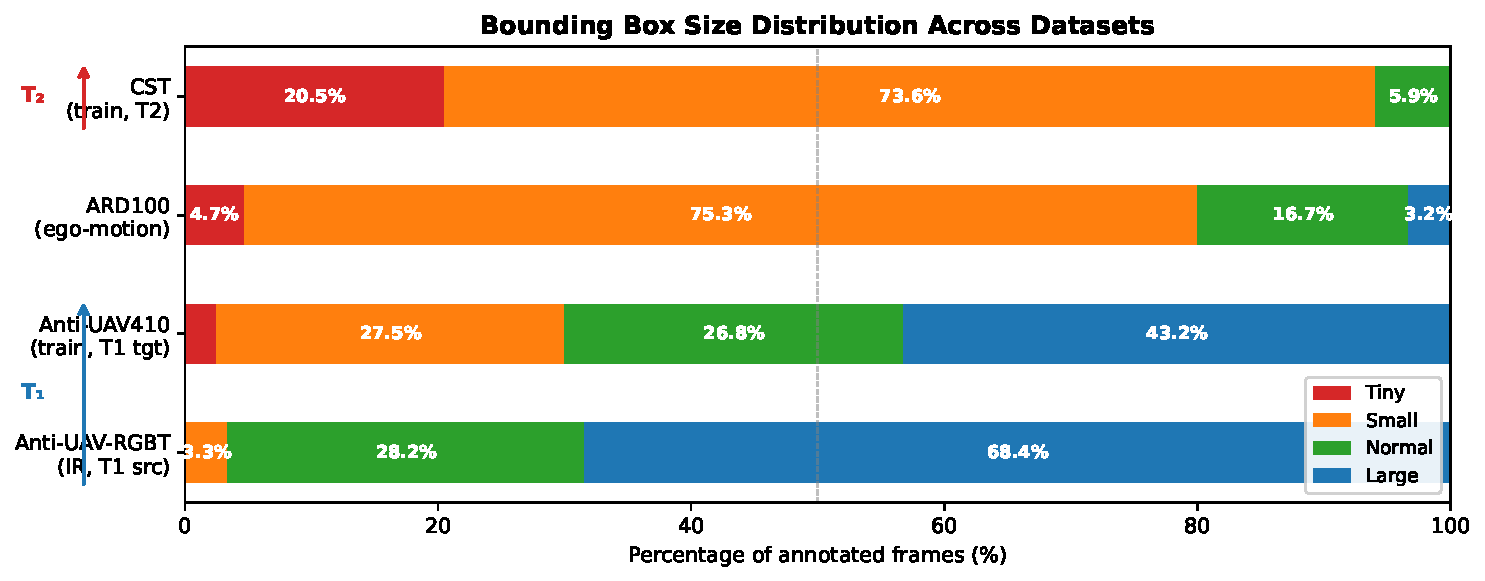
\includegraphics[width=\textwidth]{figures/fig_size_distribution.pdf}
    \caption{Bounding box size distribution across all four datasets, expressed as a percentage of annotated frames per size category. The T1 datasets (Anti-UAV-RGBT and Anti-UAV410) are dominated by large and normal targets. The T2 dataset (CST) shows a near-complete inversion: zero large targets and 94\% tiny or small targets. This scale inversion is the empirical foundation of Hypothesis H1.}
    \label{fig:size_dist}
\end{figure*}

\begin{figure*}[t]
    \centering
    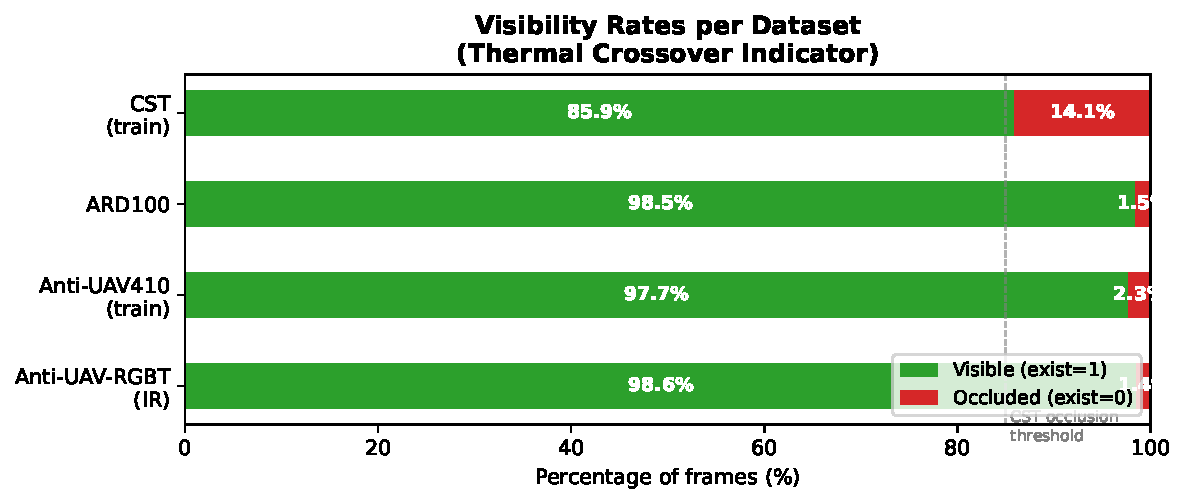
\includegraphics[width=0.85\textwidth]{figures/fig_visibility.pdf}
    \caption{Visibility and occlusion rates per dataset. CST has a substantially higher occlusion rate (14.1\%) than any T1 dataset, corresponding to the higher frequency of thermal crossover events in its acquisition conditions. The dashed line marks the CST occlusion threshold for reference.}
    \label{fig:visibility}
\end{figure*}

\begin{figure*}[t]
    \centering
    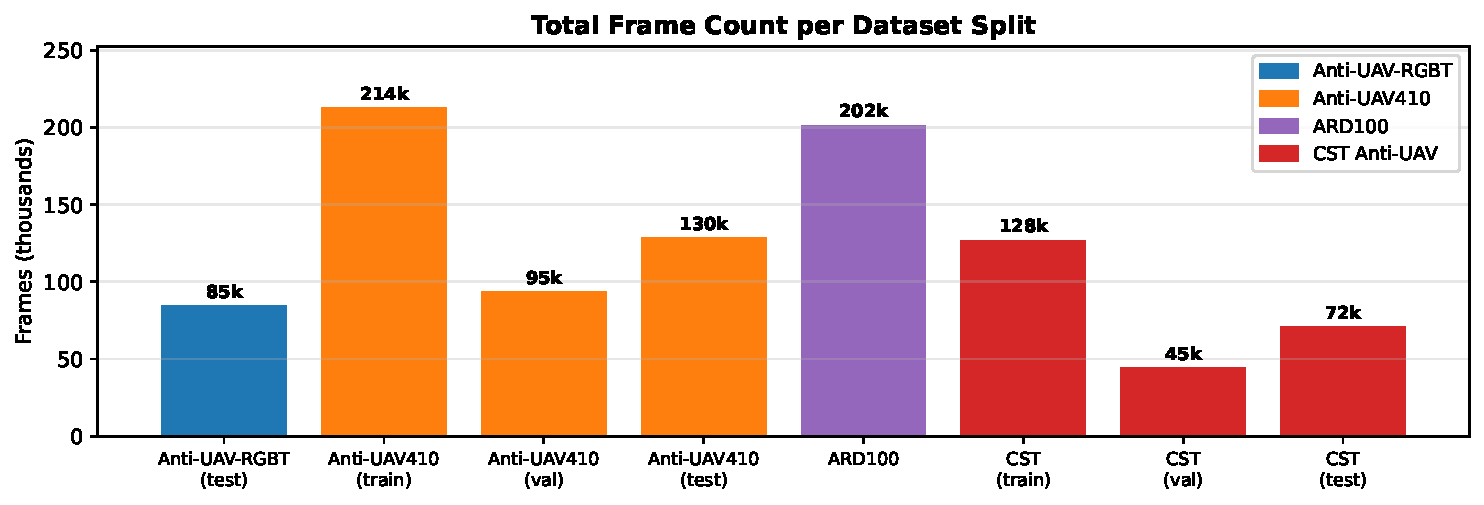
\includegraphics[width=\textwidth]{figures/fig_frame_counts.pdf}
    \caption{Total frame count per dataset split. The Anti-UAV410 training split (213,995 frames) provides the largest single-split training corpus. CST contributes 245,471 frames in total across its three splits, giving the T2 fine-tuning phase comparable data volume to T1.}
    \label{fig:frame_counts}
\end{figure*}


% ─────────────────────────────────────────────────────────────────
\subsection{Data Pipeline and Preprocessing}
\label{sec:preprocessing}
% ─────────────────────────────────────────────────────────────────

A critical infrastructure constraint shaped the data loading strategy. The project filesystem on Snellius enforces a per-project inode limit (the maximum number of file system entries, regardless of data volume). Pre-extracting all four datasets to individual JPEG frames would require approximately 1.6 million files, which exceeds this limit. An attempted extraction was aborted at sequence 27 of 160 with an inode quota error. This ruled out the conventional approach of offline frame extraction followed by standard image-folder DataLoader construction.

The adopted solution is a native-format reading strategy: all four datasets are accessed from their original storage formats during training, with no intermediate files written. For video-based datasets (Anti-UAV-RGBT and ARD100), a custom PyTorch \texttt{Dataset} class uses \texttt{cv2.VideoCapture} to decode individual frames on demand by seeking to the required timestamp. For image-based datasets (Anti-UAV410 and CST), the existing per-frame JPEG files are read directly via standard file I/O. Annotations are parsed into memory at initialization: JSON for Anti-UAV-RGBT, Anti-UAV410, and CST; Pascal VOC XML for ARD100. Frames with \texttt{exist=0} (target not visible or thermal crossover) produce empty label entries and are excluded from positive training examples but retained in the dataset iterator for occlusion analysis.

The exception is motion mask generation for ARD100. The YOLOMG backbone requires FD5 motion difference maps as a second input channel, and these must be precomputed rather than generated at runtime because they depend on a sliding window of five consecutive frames. Masks are generated once via a SLURM batch job and stored as one compressed archive per sequence to minimize inode consumption while keeping the data accessible without decompression overhead at training time.

All bounding box coordinates are normalized to the range $[0, 1]$ relative to the sensor resolution of 640$\times$512 pixels, which is consistent across all four datasets' IR streams. Boxes with width or height of zero, or with coordinates falling outside the frame boundary after normalization, are discarded. ECC homography alignment for GMC is applied per frame pair using \texttt{cv2.findTransformECC} with a maximum of 50 iterations and a termination epsilon of $10^{-5}$, operating on grayscale-converted frames.


% ─────────────────────────────────────────────────────────────────
\subsection{Training Curriculum}
\label{sec:training}
% ─────────────────────────────────────────────────────────────────

Training proceeds in three sequential stages.

In Stage 1, a source-domain baseline detector is trained on the Anti-UAV-RGBT IR stream with full supervision. This stage establishes the T1 mAP ceiling and initializes the weights used for all subsequent stages. The backbone is YOLOMG with the motion branch active from the start, using ARD100-generated FD5 masks for the motion channel alongside the IR appearance frames. The model is trained for 100 epochs using SGD with momentum 0.937 and weight decay $5 \times 10^{-4}$, with a cosine learning rate schedule decaying from an initial rate of $10^{-2}$.

In Stage 2, the T1 Teacher-Student UDA transfer is performed. The Stage 1 model is frozen as teacher. A student copy is initialized from the same weights and fine-tuned on Anti-UAV410 IR frames, supervised by teacher predictions on paired Anti-UAV-RGBT RGB frames. The student training follows the same optimizer configuration as Stage 1 but with a lower initial learning rate of $10^{-3}$ to preserve the source-domain geometry while allowing the feature extractor to adapt to TIR image statistics. The Evidential Head is attached and co-trained during this stage so that it learns the uncertainty profile of the T1 TIR domain before the scale shift is introduced.

In Stage 3, T2 continual learning fine-tuning is performed on CST. The Scale-Stratified Herding buffer populated at the end of Stage 2 is replayed at a fixed ratio of one buffer sample per four new CST samples in each mini-batch. Buffer samples are treated with the same loss terms as new samples; no separate replay weight is applied. The buffer capacity is fixed at 10\% of the total model parameter count, divided equally across the four size strata. Training runs for 50 epochs on CST, with the learning rate initialized at $5 \times 10^{-4}$ and decayed by cosine schedule.

All hyperparameter values above are based on the YOLOMG reference implementation defaults for the ARD100 setting \citep{guo_yolomg_2025} and will be tuned on the respective validation splits before final evaluation. The batch size is 16 throughout all stages.


% ─────────────────────────────────────────────────────────────────
\subsection{Evaluation Metrics}
\label{sec:metrics}
% ─────────────────────────────────────────────────────────────────

Four metrics are used, covering detection quality, temporal consistency, and the stability-plasticity trade-off.

Mean Average Precision at IoU threshold 0.5 (mAP@0.5) is computed per dataset split following the PASCAL VOC convention. It measures detection quality at each stage of the curriculum independently.

The Forgetting Measure (FM) is the primary metric for evaluating Hypothesis H1. It is defined as:
\[
    \text{FM} = \text{mAP}_{T1}^{\text{after } T2} - \text{mAP}_{T1}^{\text{after } T1}
\]
where both evaluations are conducted on the Anti-UAV410 test split. A negative FM indicates that T2 fine-tuning has caused the model to forget T1 detection capability; a larger negative value indicates more catastrophic forgetting. H1 predicts that FM will be more negative for the T2 scale shift (standard to tiny) than for the T1 modality shift (RGB to TIR), and that Scale-Stratified Herding will produce a less negative FM than flat-herding under the same 10\% memory budget.

Success Rate (SR) and Precision Rate (PR) are computed using the one-pass evaluation (OPE) protocol from the tracking community, as applied in Anti-UAV410 \citep{bohuang_410} and CST \citep{xie2025cstantiuavthermalinfrared}. SR measures the fraction of frames where the predicted bounding box overlaps the ground truth at an IoU threshold of 0.5. PR measures the fraction of frames where the predicted centre point falls within 20 pixels of the ground truth centre. Both are reported as area under the threshold curve across the full threshold range to allow comparison with published baselines.

Identity Switch count (IDSW) measures tracking consistency. The tracker is implemented as a simple IoU-based Hungarian matching algorithm \citep{aharon2022bot}, matching predicted detections to tracklets across consecutive frames. An identity switch is recorded whenever the optimal assignment changes the tracklet ID associated with a ground-truth trajectory. IDSW is reported as the total count across all test sequences and is the primary metric for evaluating the Evidential Gating module, since a well-functioning gating mechanism should suppress false detections during thermal crossover events and thereby reduce spurious ID reassignments.


% ─────────────────────────────────────────────────────────────────
\subsection{Compute Infrastructure}
\label{sec:infrastructure}
% ─────────────────────────────────────────────────────────────────

All experiments are run on Snellius, the Dutch national supercomputer operated by SURF, using the \texttt{rome} partition (AMD EPYC 7H12 nodes, 256 cores per node). GPU jobs use the A100 partition where available. The Python environment is managed via Conda (\texttt{uav\_master} environment, Python 3.10, PyTorch 2.x, CUDA 12.x). Multi-step data processing jobs are chained using SLURM's \texttt{--dependency=afterok} mechanism to enforce correct execution order. All random seeds are fixed at 42 across NumPy, PyTorch, and the Python standard library to ensure reproducibility of buffer sampling and data shuffling.


\bibliographystyle{ACM-Reference-Format}
\bibliography{references}

\end{document}
